% The 64=65 paradox: 8x8 square cut into four pieces, reassembled into a 5x13 rectangle with a thin parallelogram gap. Generated by figs_t0c07.py.
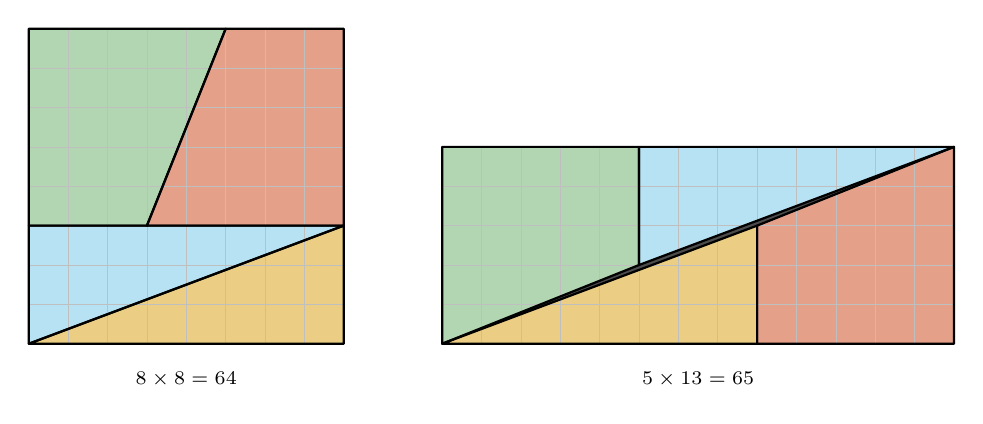
\begin{tikzpicture}[x=0.50cm,y=0.50cm,line join=round]
\fill[Goldenrod!55] (0,0) -- (8,0) -- (8,3) -- cycle;
\fill[SkyBlue!60] (0,0) -- (8,3) -- (0,3) -- cycle;
\fill[ForestGreen!35] (0,3) -- (3,3) -- (5,8) -- (0,8) -- cycle;
\fill[BrickRed!35] (3,3) -- (8,3) -- (8,8) -- (5,8) -- cycle;
\draw[gray!50,very thin] (0,0) -- (0,8);
\draw[gray!50,very thin] (1,0) -- (1,8);
\draw[gray!50,very thin] (2,0) -- (2,8);
\draw[gray!50,very thin] (3,0) -- (3,8);
\draw[gray!50,very thin] (4,0) -- (4,8);
\draw[gray!50,very thin] (5,0) -- (5,8);
\draw[gray!50,very thin] (6,0) -- (6,8);
\draw[gray!50,very thin] (7,0) -- (7,8);
\draw[gray!50,very thin] (8,0) -- (8,8);
\draw[gray!50,very thin] (0,0) -- (8,0);
\draw[gray!50,very thin] (0,1) -- (8,1);
\draw[gray!50,very thin] (0,2) -- (8,2);
\draw[gray!50,very thin] (0,3) -- (8,3);
\draw[gray!50,very thin] (0,4) -- (8,4);
\draw[gray!50,very thin] (0,5) -- (8,5);
\draw[gray!50,very thin] (0,6) -- (8,6);
\draw[gray!50,very thin] (0,7) -- (8,7);
\draw[gray!50,very thin] (0,8) -- (8,8);
\draw[black,thick] (0,0) -- (8,0) -- (8,3) -- cycle;
\draw[black,thick] (0,0) -- (8,3) -- (0,3) -- cycle;
\draw[black,thick] (0,3) -- (3,3) -- (5,8) -- (0,8) -- cycle;
\draw[black,thick] (3,3) -- (8,3) -- (8,8) -- (5,8) -- cycle;
\node[font=\scriptsize] at (4,-0.9) {$8\times8=64$};
\fill[Goldenrod!55] (10.5,0) -- (18.5,0) -- (18.5,3) -- cycle;
\fill[BrickRed!35] (18.5,0) -- (23.5,0) -- (23.5,5) -- (18.5,3) -- cycle;
\fill[ForestGreen!35] (10.5,0) -- (15.5,2) -- (15.5,5) -- (10.5,5) -- cycle;
\fill[SkyBlue!60] (15.5,2) -- (23.5,5) -- (15.5,5) -- cycle;
\draw[gray!50,very thin] (10.5,0) -- (10.5,5);
\draw[gray!50,very thin] (11.5,0) -- (11.5,5);
\draw[gray!50,very thin] (12.5,0) -- (12.5,5);
\draw[gray!50,very thin] (13.5,0) -- (13.5,5);
\draw[gray!50,very thin] (14.5,0) -- (14.5,5);
\draw[gray!50,very thin] (15.5,0) -- (15.5,5);
\draw[gray!50,very thin] (16.5,0) -- (16.5,5);
\draw[gray!50,very thin] (17.5,0) -- (17.5,5);
\draw[gray!50,very thin] (18.5,0) -- (18.5,5);
\draw[gray!50,very thin] (19.5,0) -- (19.5,5);
\draw[gray!50,very thin] (20.5,0) -- (20.5,5);
\draw[gray!50,very thin] (21.5,0) -- (21.5,5);
\draw[gray!50,very thin] (22.5,0) -- (22.5,5);
\draw[gray!50,very thin] (23.5,0) -- (23.5,5);
\draw[gray!50,very thin] (10.5,0) -- (23.5,0);
\draw[gray!50,very thin] (10.5,1) -- (23.5,1);
\draw[gray!50,very thin] (10.5,2) -- (23.5,2);
\draw[gray!50,very thin] (10.5,3) -- (23.5,3);
\draw[gray!50,very thin] (10.5,4) -- (23.5,4);
\draw[gray!50,very thin] (10.5,5) -- (23.5,5);
\fill[black!70] (10.5,0) -- (18.5,3) -- (23.5,5) -- (15.5,2) -- cycle;
\draw[black,thick] (10.5,0) -- (18.5,0) -- (18.5,3) -- cycle;
\draw[black,thick] (18.5,0) -- (23.5,0) -- (23.5,5) -- (18.5,3) -- cycle;
\draw[black,thick] (10.5,0) -- (15.5,2) -- (15.5,5) -- (10.5,5) -- cycle;
\draw[black,thick] (15.5,2) -- (23.5,5) -- (15.5,5) -- cycle;
\node[font=\scriptsize] at (17.0,-0.9) {$5\times13=65$};
\end{tikzpicture}
